\documentclass[submit,techrep,noauthor]{ipsj}
%\documentclass[submit,techrep,noauthor]{jreport}
\usepackage{otf}
\usepackage[T1]{fontenc}
\usepackage{lmodern}
\usepackage{textcomp}
\usepackage{latexsym}
\usepackage[dvipdfmx]{graphicx}
\usepackage{color}
\usepackage{listings,jvlisting}
\usepackage[many]{tcolorbox}
\usepackage{ascmac}
\usepackage{subfigure}
\usepackage{colortbl,array,xcolor}
\usepackage{multirow}
\usepackage{booktabs}

\lstset{
  language={java},
  basicstyle={\ttfamily},
  identifierstyle={\small},
  commentstyle={\smallitshape},
  keywordstyle={\small\bfseries},
  ndkeywordstyle={\small},
  stringstyle={\small\ttfamily},
  frame={tb},
  breaklines=true,
  columns=[l]{fullflexible},
  numbers=left,
  xrightmargin=0zw,
  xleftmargin=3zw,
  numberstyle={\scriptsize},
  stepnumber=1,
  numbersep=1zw,
  lineskip=-0.5ex
}

\definecolor{dgreen}{rgb}{0.1,0.5,0.1}

\def\Underline{\setbox0\hbox\bgroup\let\\\endUnderline}
\def\endUnderline{\vphantom{y}\egroup\smash{\underline{\box0}}\\}
\def\|{\verb|}
\def\newblock{\hskip .11em plus .33em minus .07em}
\newcommand{\smallsection}[1]{\noindent\textbf{#1.}}
\renewcommand{\lstlistingname}{プログラム}

\def\summarybox#1#2{
\medskip
\begin{tcolorbox}[enhanced,title=#1, attach boxed title to top left= {xshift=0mm, yshift*=-\tcboxedtitleheight/2}]
    #2
\end{tcolorbox}
}

\begin{document}


\title{OSSにおけるJavaのレコード・クラス利用実態の初期調査}

%\etitle{English Title}

\affiliate{KU}{九州大学\\
Kyushu University}

\author{杉原 裕太}{}{KU}[sugihara@posl.ait.kyushu-u.ac.jp]
\author{近藤 将成}{}{KU}[kondo@ait.kyushu-u.ac.jp]
\author{亀井 靖高}{}{KU}[kamei@ait.kyushu-u.ac.jp]
\author{鵜林 尚靖}{}{KU}[ubayashi@ait.kyushu-u.ac.jp]

\begin{abstract}
  今日広く利用されているプログラミング言語であるJavaは,円滑なコーディングを目的として新たな言語仕様を導入することがある.
  過去のJava言語アップデートでもジェネリクスやラムダ式といった言語仕様が追加されており,これらがリファクタリングにどのように活用可能であるのか研究されてきた.
  そして2021年に追加された言語仕様であるレコード・クラスは,一部の型宣言を簡潔に行うことを可能とし,ソースコード記述量の削減に寄与すると考えられている.
  しかしながら,レコード・クラスに関して,リファクタリング上の恩恵を報告する研究はまだ行われていない.
  そこで本稿ではレコード・クラスのリファクタリング利用に関する初期調査として,GitHub上のOSSにおけるレコード・クラスの利用実態を評価した.
  その結果,データセットとして取得した2000件のレポジトリのうち,70件のレポジトリで合計3244のレコード・クラスが定義されていることがわかった.
  また,コミットによるレコード・クラスの追加のうち,22.2\%が既存クラスをレコード・クラスに変更するリファクタリングであることがわかった.
\end{abstract}

\begin{jkeyword}
  Java,レコード・クラス,リファクタリング
\end{jkeyword}

\maketitle

\setcounter{page}{1}

{\large
%1 はじめに
\section{はじめに\label{intro}}

今日広く利用されているプログラミング言語であるJavaは,円滑なコーディングを目的として新たな言語仕様を導入することがある.
過去のJava言語アップデートでもジェネリクスやラムダ式といった言語仕様が追加されており,これらが開発者たちによってどのように利用されているのか,そしてコーディング作業上でどのような恩恵をもたらすのか調査が行われてきた\cite{Generics_Research}\cite{Lambda_Research}.
そして2021年3月のアップデートであるJava16で,Javaはレコード・クラス(以下レコードと記述)という新たな言語仕様を導入した.
レコードはイミュータブルな値ベース・クラスの宣言を簡潔に行うことを可能とし,ソースコード記述量の削減に寄与すると考えられている.
しかしながら,レコードに関して,開発者たちによる利用およびコーディング上の恩恵を報告する研究はまだ行われていない.
そこで本稿ではレコードの利用に関する初期調査として,GitHub上のOSSにおけるレコードの利用実態を評価した.
本稿における調査の目的として,次のようなものを掲げている.
\begin{quote}
  \begin{itemize}
    \item Java言語を利用する開発者に対し,レコードの適切な利用を推進する.
    \item Java言語の開発者に対し,言語仕様デザインのヒントを提供する.
    \item レコードを用いたリファクタリングの支援を行うツール開発にあたり,必要な知見を収集する.
  \end{itemize}
\end{quote}

そして,上記の目的に基づき,次の4つのRQを設定している.
\begin{itemize}
  \item[RQ1 : ] レコードはOSSにおいて,どの程度の数使用されているのか?
  \item[RQ2 : ] 使用されているレコードの特徴はどのようになっているか?
  \item[RQ3 : ] クラスをレコードに変更するリファクタリングでは,どの程度の恩恵を享受できるのか?
  \item[RQ4 : ] クラスからレコードへの変更を阻害する要因は何か?
\end{itemize}

本稿では,\ref{motivation}節でレコードの仕様を含めた背景と,動機について述べる.
\ref{methodology}節でデータセットと手法について説明し,\ref{result}節で各RQに対する結果を述べる.
最後に\ref{threats}節で妥当性の脅威,\ref{conclusion}節でまとめを述べる.
%2 動機
\section{背景と動機\label{motivation}}

\subsection{レコードの仕様\label{record_specification}}

\begin{figure}[t]
\begin{lstlisting}
record Point(int x, int y) { }
\end{lstlisting}
\caption{レコードの宣言}
\label{record_decl}
\end{figure}

\begin{figure}[t]
\begin{lstlisting}
final class Point {
    private final int x;
    private final int y;

    public Point(int x, int y) {
        this.x = x;
        this.y = y;
    }

    public int x() { return x; }
    public int y() { return y; }

    @Override
    public boolean equals(Object o) {
        if(o instanceof Point p){
            return p.x == x && p.y == y;
        }
        return false;
    }

    @Override
    public int hashCode() {
        return java.util.Objects
            .hash(x, y);
    }

    @Override
    public String toString() {
        return "Point[x=%d, y=%d]"
            .formatted(x, y);
    }
}
\end{lstlisting}
\caption{\figref{record_decl}と等価なクラス宣言}
\label{class_decl}
\end{figure}

レコードとは,不変な変数群を保持することを目的として作られた型宣言のフレームワークであり,2021年3月のJava16(プレビューはJava14から)でJavaに登場した\cite{Record_Purpose}.
レコードの宣言では,クラス宣言の際に用いるキーワードclassの代わりに,文脈的キーワードのrecordを用いる.
そして\figref{record_decl}のように,レコード名の直後にヘッダ(レコードの保持するフィールドのリスト)を宣言する.
これらによって次のメンバが暗黙的に実装され,利用できるようになる.

\begin{quote}
    \begin{itemize}
        \item ヘッダに対応するprivateかつfinalなインスタンスフィールド
        \item カノニカルコンストラクタ(ヘッダと同じ型の順番で引数をとり,対応する各フィールドを初期化するコンストラクタ)
        \item 各フィールドと同じ名前をもつゲッタメソッド
        \item 一定の規則に基づいて構成されたtoString/equals/hashCodeメソッド
    \end{itemize}
\end{quote}


参考として\figref{class_decl}に,\figref{record_decl}のレコードと等価であるクラス宣言を示す.
レコードは,\figref{class_decl}のような値ベース・クラスを簡潔に宣言することを可能とし,ソースコード記述量の削減に効果を発揮すると考えられる.
また,ソースコードの読み手がレコードの仕様を理解している場合,レコード型宣言の提供するインタフェースを素早く理解することができるという恩恵もある.
なお,暗黙的に実装されたメソッドおよびコンストラクタは,同じシグネチャでレコードの内部に改めて宣言することで,オーバーライドすることも可能である.

レコードの宣言には,通常クラスに存在しない次のような制約も課される\cite{JLS17}.

\begin{quote}
    \begin{itemize}
        \item クラスを継承できない.(インタフェースの実装は可.)
        \item クラスの継承元になれない.
        \item ヘッダとは別のインスタンスフィールドを宣言できない.
        \item インスタンスイニシャライザを宣言できない.
        \item カノニカルコンストラクタをオーバーライドしないコンストラクタは,最初に必ずカノニカルコンストラクタを呼び出さないといけない.
    \end{itemize}
\end{quote}

継承の制約やインスタンスフィールドの制約は,レコードの不変性を保証するためのものである.
インスタンスイニシャライザとコンストラクタの制約は,レコードの初期化がカノニカルコンストラクタによって確実に行われることを保証するためのものである.

\subsection{Javaの言語仕様に対して過去に行われた調査\label{related_works}}
\subsubsection{Javaのジェネリクスに関する研究\label{generics_research}}
Chrisらは,Java5で追加された言語仕様であるジェネリクスについて,OSSにおける利用の調査を行った\cite{Generics_Research}.
ジェネリクスは,クラスあるいはメソッド中の型宣言に自由度を持たせる言語仕様であり,ダウンキャスト式などのアンチパターンの減少に効果を発揮するとされている.
本関連研究ではOSSの開発履歴を解析し,ジェネリクスのもたらす効果の検証とともに,利用数の変遷やジェネリクスに与えられやすい型引数などの統計を取得している.

データセットは,Javaにジェネリクスが導入される以前に開始した20のOSSと,Javaにジェネリクスが導入されたより後に開始した20のOSSである.
結果として,アンチパターンの減少の側面からは,ジェネリクスの適用数の増加に伴って統計学的有意にダウンキャスト式の割合が減少していることがわかった.
利用の側面からは,ジェネリクス導入以前に開始したOSSのうち15件で,ジェネリクス導入以降に開始したOSSのうち全てで,ジェネリクスが利用されていることがわかった.
また,ジェネリクスの型引数としては,String型が最も多く与えられていることがわかった.

\subsubsection{Javaのラムダ式に関する研究\label{lambda_research}}
DavoodとAmeyaらは,Java8で追加された言語仕様であるラムダ式について,OSSにおける利用に関する調査を行った\cite{Lambda_Research}.
Javaにおけるラムダ式は,関数をオブジェクトのように扱うことができる言語仕様であり,同等の機能を提供する無名クラスをより簡潔に記述したものである.
本関連研究ではOSSの開発履歴を解析し,ラムダ式の利用を関数型インタフェースや導入目的などの側面から分析している.

データセットは,GitHubから収集したスター数トップ2,000のJavaのOSSである.
結果として,利用数の側面からは,2,000件中241件のリポジトリで,合計100,540件のラムダ式が利用されていることがわかった.
また,2016年内において追加されたコードに含まれるラムダ式の割合は2015年の3倍程度になっており,ラムダ式の増加が加速していることがわかった.
リファクタリング利用の側面からは,51件のコミットを選定して調査したところ,5,855件のラムダ式が無名クラスの置き換えで導入されていたことがわかった.

\subsection{本研究の目的\label{research_goals}}
\ref{related_works}節の2つの研究では,言語仕様の利用数および適用数の増加について調査が行われている.
また,言語仕様の利用形態に関する俯瞰として,\ref{generics_research}節の研究ではジェネリクスに与えられる型引数について,\ref{lambda_research}節の研究ではラムダ式の型として与えられる関数型インタフェースの利用について調査されていた.
よって,RQ1およびRQ2では,これらの関連研究に倣って,以下のような調査を行う.
\begin{itemize}
    \item[RQ1 : ] レコードの利用における全体的な俯瞰を与えるため,OSSにおけるレコードの適用数やその変遷を調査する.
    \item[RQ2 : ] レコードの利用形態に関する俯瞰として,レコードの要素型と実装インタフェースについて統計を取得する.
\end{itemize}

また,本研究ではレコードを用いたリファクタリングを支援するツールの開発のために,必要な知見を収集することを目的としている.
よってRQ3およびRQ4では,より効果的な支援の提供のため,レコードを用いたリファクタリングについて以下の調査を行う.
\begin{itemize}
    \item[RQ3 : ] レコードを用いたリファクタリングで,ソースコードの要素削減の観点からどの程度の恩恵があるのか明らかにする.
    \item[RQ4 : ] レコードを用いたリファクタリングを適用するにあたり,\ref{record_specification}節で挙げたような制約も含め,どのような障害があるのか明らかにする.
\end{itemize}
%3 実験方法
\section{データセットと手法\label{methodology}}

\subsection{データセット}
データセットとなるOSSは,GitHubの検索用URLを用いたスクレイピングで,2022年12月24日から25日にかけて収集した.
以下の条件のもと,スター数の多い順に2,000件のリポジトリを選択している.
\begin{itemize}
    \item[(1) ] リポジトリの言語がJavaである.
    \item[(2) ] 最終プッシュが2020年3月17日以降である.
\end{itemize}
(2)の2020年3月17日は,レコードがプレビュー機能として実装されたJava14のリリース日である.
この条件は,レコードが含まれている可能性の低いリポジトリを除外する目的で設定している.

\subsection{手法}
各RQにおける解析は,リポジトリ中の.javaファイルから抽象構文木を生成して行った.
抽象構文木の生成に用いたのは,Java17APIのパッケージcom.sun.source.treeのインターフェース群をベースにして制作した独自のパーサである.
独自のパーサを用いた理由は,レコードがJava16以降の言語仕様であり,対応するバージョンがJava15までであるJavaParserなどでは解析できない可能性を考慮したからである.

\subsubsection{RQ1\label{rq1_method}}
RQ1については,はじめにリポジトリをクローンした時点(2022年12月25日)でのレコードの利用数を集計した.
それからデータセット中の各リポジトリを,2020年4月から2022年12月の期間で各月1日時点のコミットに巻き戻し,レコードの利用数を集計した.

\subsubsection{RQ2\label{rq2_method}}
RQ1の結果,71件のリポジトリでレコードの使用履歴がみられた.
よってRQ2では,これら71件のリポジトリに含まれるレコードに対して,ヘッダ及び実装インタフェースの情報の取得を行った.
さらに同じリポジトリ群に含まれるクラスについても,インスタンスフィールド及び実装インタフェースの情報を取得し,結果を比較した.
なお,フィールド型およびインタフェースは,アノテーションを除去した文字列ベースで分類している.

\subsubsection{RQ3\label{rq3_method}}
RQ3では,レコードの追加・削除について統計を取るため,各リポジトリに対して次の操作を行った.
\begin{itemize}
    \item[(1) ] git diffコマンドで,親コミットから変更されたファイルのパスを取得する.
    \item[(2) ] (1)のファイルが存在する場合,ファイルに含まれる型のクラスパスと型の情報を取得する.存在しない場合,削除ファイルとして記録する.
    \item[(3) ] 親コミットに遡上する.
    \item[(4) ] (1)のファイルが存在する場合,型のクラスパスと型の情報を取得する.存在しない場合,追加ファイルとして記録する.
    \item[(5) ] (2)と(4)の情報を比較する.
\end{itemize}
上記の操作を繰り返していき,レコードの追加および削除の件数を集計した.
さらに,クラスからレコードの変更については,コンストラクタ,ゲッタメソッド,toString/equals/hashCodeメソッド,その他メソッドの増減についても集計した.
なお,ここでいうゲッタメソッドは,名前がインスタンスフィールド名,あるいはインスタンスフィールド名に接頭辞getを付けたのものであり,引数のないメソッドとしている.
また,toString/equals/hashCodeの各メソッドはシグネチャで判定している.

\subsubsection{RQ4\label{rq4_method}}
RQ3を実施する過程で,クラスからレコードへのリファクタリングを一度に50件以上行うコミットを複数発見した.
RQ4における1つ目の調査では,これらのコミットを目視調査することで,リファクタリング作業に伴うコストについて紐解いていく.
また,同じくRQ3の過程で,レコードからクラスに変更されたケースを31件検出した.
これらの変更は,レコードの利用で何かしらの弊害があったから行われた可能性がある.
そしてレコードの利用による弊害は,開発者がレコードの導入を渋る理由の一端を担っている可能性があり,今後のリファクタリングツールの設計の上で重要な要素になると考えられる.
よってRQ4における2つ目の調査では,レコードからクラスへの変更についてソースコードの差分やコメント,GitHub上の議論を目視し,理由を調査した.
%4 実験結果と考察
\section{実験結果と考察\label{result}}

\subsection{RQ1 : レコードはOSSにおいて,どの程度の数使用されているのか?\label{rq1_result}}

\begin{figure}[t]
    \centering
    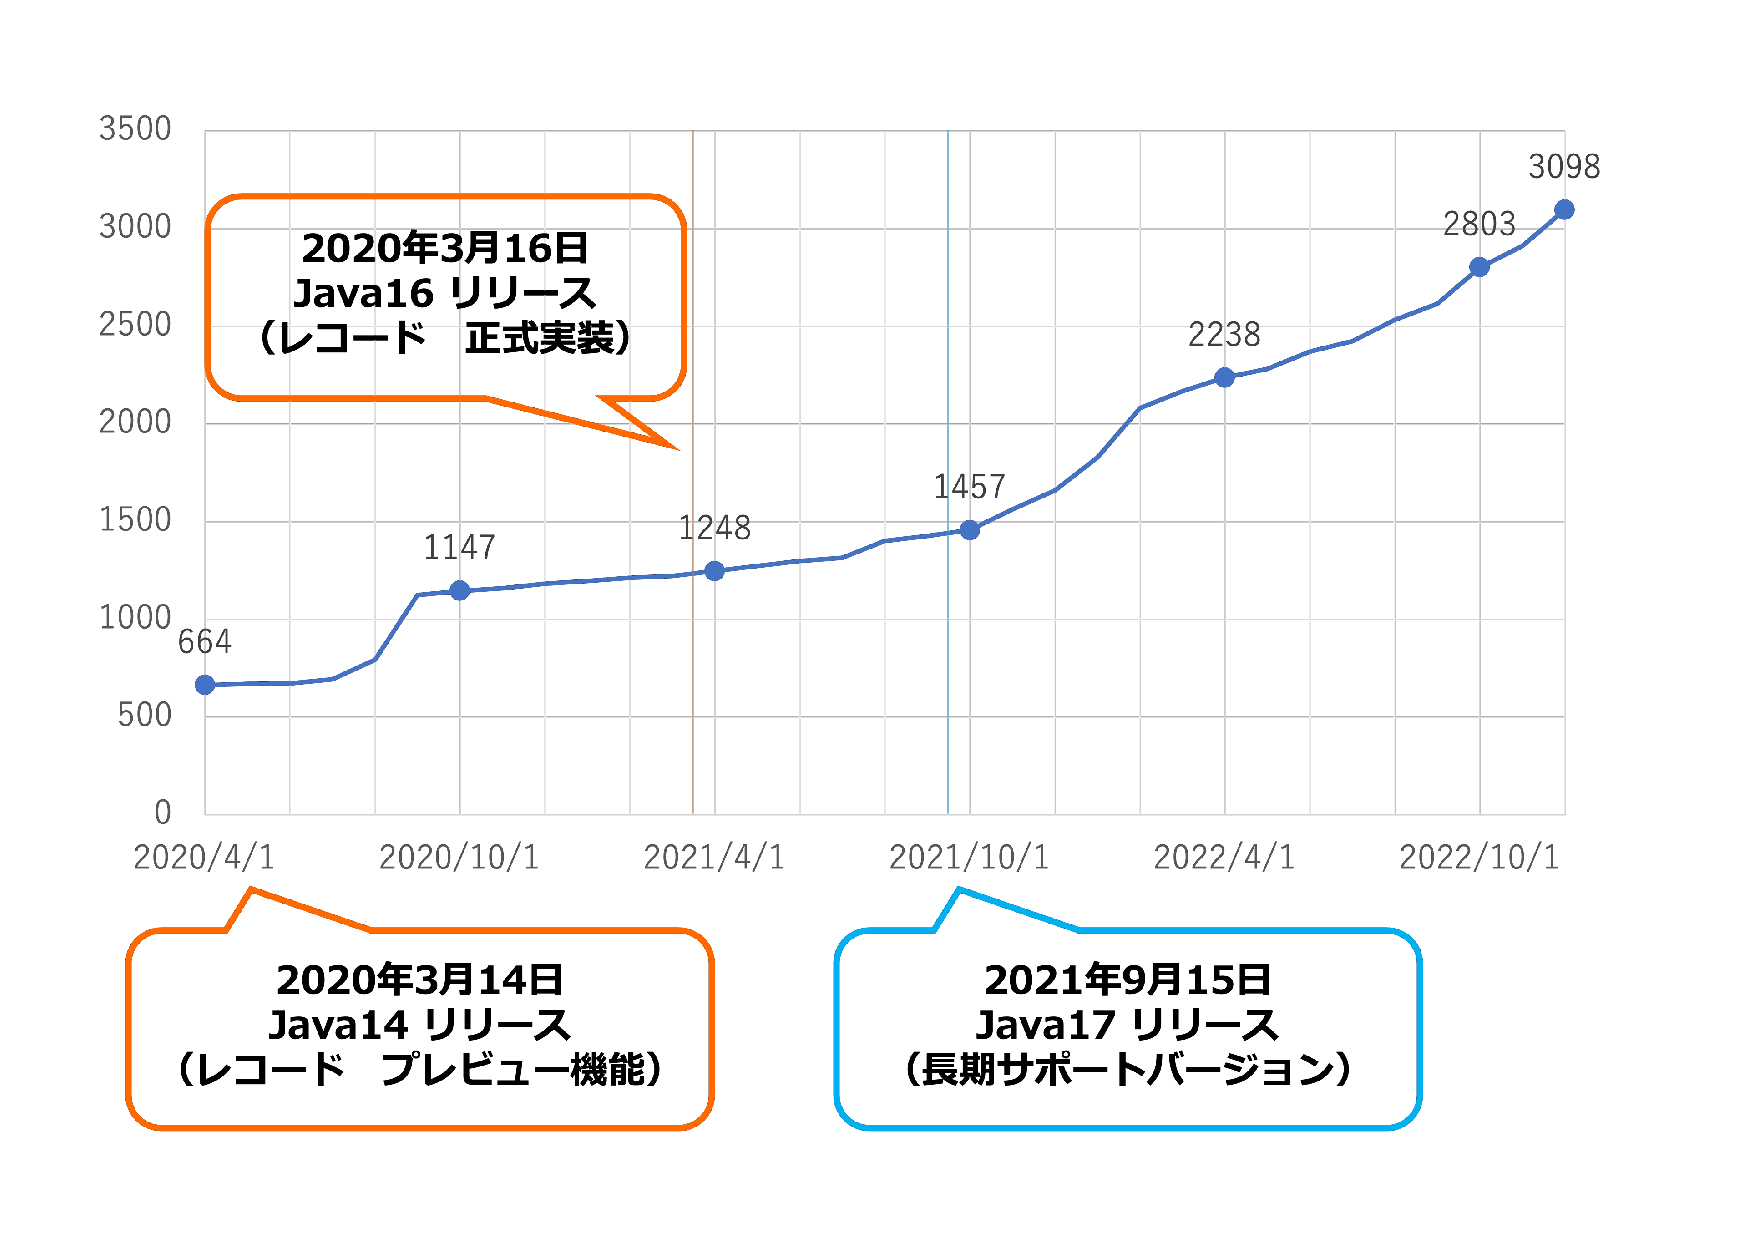
\includegraphics[width=10cm]{image/num_records.pdf}
    \caption{レコードの利用数の変遷}
    \label{num_records}
\end{figure}

\figref{num_records}は,2020年4月から2022年12月までのレコード利用数の変遷を示した折れ線グラフである.
データセットのレポジトリをクローンした2022年12月25日時点では,70件のレポジトリで合計3,244件のレコードが利用されていた.
利用数の伸び方に注目してみると,Java17がリリースされる2020年9月までの18か月の区間は月44.1件のペース,2020年10月以降の14か月の区間は月117.2件のペースでレコードが導入されている.
すなわち,レコードの利用数の伸びはJava17の登場以降に加速していることがわかる.

\subsection{RQ2 : 使用されているレコードの特徴はどのようになっているか?\label{rq2_result}}
\subsubsection{インスタンスフィールド数\label{num_instance_fields}}

\begin{table}[t]
    \caption{定義フィールド個数別のレコード(クラス)の件数}
    \label{num_fields}
    \centering
    \begin{tabular}{c||r|r|r|r}
        \hline
        フィールド数 & \multicolumn{2}{c|}{レコード} & \multicolumn{2}{c}{クラス}\\
         & 個数 & 割合 & 個数 & 割合\\
        \hline\hline
        0 & 317 & 9.8\% & 229,275 & 60.9\%\\
        1 & 815 & 25.1\% & 54,129 & 14.4\%\\
        2 & 1,070 & 33.0\% & 32,501 & 8.6\%\\
        3 & 483 & 14.9\% & 19,358 & 5.1\%\\
        4 & 205 & 6.3\% & 12,043 & 3.2\%\\
        5 & 129 & 4.0\% & 8,115 & 2.2\%\\
        6\textasciitilde10 & 157 & 4.8\% & 15,174 & 4.0\%\\
        11\textasciitilde & 68 & 2.1\% & 6,077 & 1.6\%\\
        \hline
        合計 & 3,244 & - & 376,672 & - \\
        \hline
    \end{tabular}
\end{table}

\tabref{num_fields}は,レコードおよびクラスのインスタンスフィールド数別に,件数を集計したものである.
最も多かったのはフィールド数が2個のレコードで,全体の33.0\%を占めていた.
なお,定義1件あたりのフィールド数を算出したとことろ,クラスは1.85個であるのに対し,レコードは2.88個であった.
すなわち,レコードの方がクラスよりも多くのフィールドを持つことがわかった.

\subsubsection{フィールド型の傾向\label{field_type_trend}}

\begin{table}[t]
    \caption{レコードのフィールド型の傾向}
    \label{record_field_types}
    \centering
    \begin{tabular}{c||r|r}
        \hline
        型名 & 個数 & 割合\\
        \hline\hline
        int & 2,871 & 30.7\%\\
        (java.lang.)String & 1,725 & 18.4\%\\
        long & 615 & 6.6\%\\
        boolean & 374 & 4.0\%\\
        double & 205 & 2.2\%\\
        List<String> & 109 & 1.2\%\\
        (java.lang.)Boolean & 74 & 0.8\%\\
        double[] & 68 & 0.7\%\\
        (java.lang.)Object & 65 & 0.7\%\\
        (java.lang.)Integer & 64 & 0.7\%\\
        その他 & 3,182 & 34.0\%\\
        \hline
        合計 & 9,352 & -\\
        \hline
    \end{tabular}
\end{table}

\begin{table}[t]
    \caption{クラスのフィールド型の傾向}
    \label{class_field_types}
    \centering
    \begin{tabular}{c||r|r}
        \hline
        型名 & 個数 & 割合\\
        \hline\hline
        long & 205,434 & 29.4\%\\
        int & 77,043 & 11.0\%\\
        (java.lang.)String & 53,182 & 7.6\%\\
        boolean & 39,275 & 5.6\%\\
        (java.lang.)Object & 5,829 & 0.8\%\\
        double & 4,408 & 0.6\%\\
        byte[] & 3,875 & 0.6\%\\
        List<String> & 3,501 & 0.5\%\\
        int[] & 3,398 & 0.5\%\\
        float & 3,246 & 0.5\%\\
        その他 & 298,946 & 42.8\%\\
        \hline
        合計 & 698,137 & - \\
        \hline
    \end{tabular}
\end{table}

% \begin{table}[t]
%     \caption{レコード(クラス)のフィールド型の傾向}
%     \label{field_types}
%     \centering
%     \begin{tabular}{c||r|r||c||r|r}
%         \hline
%         型名 & \multicolumn{2}{c||}{レコード} & 型名 &\multicolumn{2}{c|}{クラス}\\
%          & 個数 & 割合 & & 個数 & 割合\\
%         \hline\hline
%         int & 2,871 & 30.7\% & long & 205,434 & 29.4\%\\
%         (java.lang.)String & 1,725 & 18.4\% & int & 77,043 & 11.0\%\\
%         long & 615 & 6.6\% & (java.lang.)String & 53,182 & 7.6\%\\
%         boolean & 374 & 4.0\% & boolean & 39,275 & 5.6\%\\
%         double & 205 & 2.2\% & (java.lang.)Object & 5,829 & 0.8\%\\
%         List<String> & 109 & 1.2\% & double & 4,408 & 0.6\%\\
%         (java.lang.)Boolean & 74 & 0.8\% & byte[] & 3,875 & 0.6\%\\
%         double[] & 68 & 0.7\% & List<String> & 3,501 & 0.5\%\\
%         (java.lang.)Object & 65 & 0.7\% & int[] & 3,398 & 0.5\%\\
%         (java.lang.)Integer & 64 & 0.7\% & float & 3,246 & 0.5\%\\
%         その他 & 3,182 & 34.0\% & その他 & 298,946 & 42.8\%\\
%         \hline
%         合計 & 9,352 & - & 合計 & 698,137 & - \\
%         \hline
%     \end{tabular}
% \end{table}

% \begin{table}[t]
%     \caption{レコード(クラス)のフィールド型の傾向(種類別)}
%     \label{field_type_attributes}
%     \centering
%     \begin{tabular}{c||r|r|r|r}
%         \hline
%         型の種類 & \multicolumn{2}{c|}{レコード} & \multicolumn{2}{c}{クラス}\\
%          & 個数 & 割合 & 個数 & 割合\\
%         \hline\hline
%         プリミティブ型計 & 4,199 & 44.9\% & 333,636 & 47.8\%\\
%         プリミティブ配列型計 & 160 & 1.7\% & 14,400 & 2.1\%\\
%         ラッパークラス型計 & 224 & 2.4\% & 6,653 & 1.0\%\\
%         セット型計 & 95 & 1.0\% & 4,861 & 0.7\%\\
%         リスト型計 & 339 & 3.6\% & 19,217 & 2.8\%\\
%         マップ型計 & 158 & 1.7\% & 11,824 & 1.7\%\\
%         \hline
%     \end{tabular}
% \end{table}

\tabref{record_field_types}はレコードのインスタンスフィールド型,\tabref{class_field_types}はクラスのインスタンスフィールド型の傾向を集計したものである.
型の中にはjava.lang.Stringのように完全限定名で指定されているものもあったので,それらも単純名での検出と一緒にして計上している.
結果をみると,レコードのフィールド型として際立って利用されているのはint型であり,全体の30.7\%を占めている.
対してクラスのフィールド型として際立っているのはlong型であり,全体の29.4\%を占めている.
ただしこの数値は,レポジトリSapMachineとJetBrainsRuntimeにおける,大量のlong型フィールドを含むクラス群を計上した結果である.
これらのレポジトリには,わずか2つで合計81,903ものlong型フィールド宣言(全long型フィールドの39.9\%)を行うクラスが含まれており,結果に大きな影響を与えている.

SapMachineとJetBrainsRuntimeを除いた場合,レコードのフィールド型で最も多いのはStringで1,410件(全体の22.6\%),次点はintで1,177件(全体の18.9\%)となる.
一方,クラスのフィールド型で最も多いのはintで41,969件(全体の13.1\%),次点はStringで35,687件(全体の11.2\%)となる.

% そして\tabref{field_types_attributes}は,フィールド型を分類して集計したものである.
% Javaコレクションフレームワークの分類\cite{Collections_Framework}を参考にし,セット型はSet,HashSet,TreeSet,LinkedHashSetの4つ,リスト型はList,ArrayList,LinkedListの3つ,マップ型はMap,HashMap,TreeMap,LinkedHashMapの4つとしている.
% また,ジェネリクス及びrawタイプは区別していない.


\subsubsection{実装インタフェース数\label{num_implemented_interfaces}}

\begin{table}[t]
    \caption{実装インタフェース数別のレコード(クラス)の件数}
    \label{num_interfaces}
    \centering
    \begin{tabular}{c||r|r|r|r}
        \hline
        インタフェース数 & \multicolumn{2}{c|}{レコード} & \multicolumn{2}{c}{クラス}\\
         & 件数 & 割合 & 件数 & 割合\\
        \hline\hline
        0 & 2,443 & 75.3\% & 309,354 & 82.1\%\\
        1 & 743 & 22.9\% & 58,507 & 15.5\%\\
        2 & 54 & 1.7\% & 6,719 & 1.8\%\\
        3 & 4 & 0.1\% & 1,430 & 0.4\%\\\
        4\textasciitilde & 0 & 0.0\% & 662 & 0.2\%\\
        \hline
        合計 & 3,244 & - & 376,672 & - \\
        \hline
    \end{tabular}
\end{table}

\tabref{num_interfaces}は,レコードおよびクラスの実装インタフェース数別に,件数を集計したものである.
実装インタフェース数の平均をとると,レコードは0.266,クラスは0.213であるので,レコードの方がインタフェースの実装が行われやすいということがわかった.

\subsubsection{実装インタフェースの傾向\label{interface_trend}}

\begin{table}[t]
    \caption{レコードの実装インタフェースの傾向}
    \label{record_interface_types}
    \centering
    \begin{tabular}{c||r|r}
        \hline
        型名 & 件数 & 割合\\
        \hline\hline
        (java.io.)Serializable & 253 & 29.3\%\\
        Writeable & 49 & 5.7\%\\
        Decoration & 35 & 4.1\%\\
        Comparable & 34 & 3.9\%\\
        ToXContentObject & 30 & 3.5\%\\
        ThrowingExternalizable & 26 & 3.0\%\\
        ClusterStateTaskListener & 16 & 1.9\%\\
        ExpirationPolicyBuilder & 16 & 1.9\%\\
        ToXContentFragment & 15 & 1.7\%\\
        Runnable & 14 & 1.6\%\\
        その他 & 375 & 43.5\%\\
        \hline
        合計 & 863 & -\\
        \hline
    \end{tabular}
\end{table}

\begin{table}[t]
    \caption{クラスの実装インタフェースの傾向}
    \label{class_interface_types}
    \centering
    \begin{tabular}{c||r|r}
        \hline
        型名 & 個数 & 割合\\
        \hline\hline
        (java.io.)Serializable & 4,242 & 5.3\%\\
        Runnable & 3,225 & 4.0\%\\
        (java.util.)Iterator & 1,343 & 1.7\%\\
        (java.lang.)Comparable & 1,034 & 1.3\%\\
        (java.lang.)Cloneable & 888 & 1.1\%\\
        Collector & 811 & 1.0\%\\
        Writeable & 790 & 1.0\%\\
        ActionListener & 740 & 0.9\%\\
        ToXContentObject & 721 & 0.9\%\\
        IdentifiedDataSerializable & 606 & 0.8\%\\
        その他 & 65,649 & 82.0\%\\
        \hline
        合計 & 80,049 & -\\
        \hline
    \end{tabular}
\end{table}

\tabref{record_field_types}はレコードのインスタンスフィールド型,\tabref{class_field_types}はクラスのインスタンスフィールド型の傾向を集計したものである.
こちらも\ref{field_type_trend}節と同じく,完全限定名の指定と単純名の指定をまとめてある.また,型引数のある型は型引数を無視してまとめてある(rawタイプも含む).
結果を見ると,レコードもクラスも最も多く実装されているのは(java.io.)Serializableとなった.
ただ全体で見た比率に差があり,レコードは7.8\%,クラスは1.1\%への実装となっている.
クラスのみへの実装が際立っているインタフェースとしてはRunnableが挙げられる.
レコードにおいては全体の0.4\%程度だが,クラスでは全体の0.9\%となっている.

\subsection{RQ3 : クラスをレコードに変更するリファクタリングでは,どの程度の恩恵を享受できるのか?\label{rq3_result}}

\subsubsection{レコードの追加と削除の件数}
コミットで変更されたファイルの履歴からレコードの追加と削除を抽出し,分類を行った.
なお,ラムダ式などの内部で宣言されているレコードはクラスパスが生成できず,差分間で同一の型を特定するのが困難であるので,ここではトップレベルレコード及びクラス内部レコードのみを対象としている.
\tabref{record_addition}にレコードの追加の内訳,\tabref{record_addition}にレコードの削除の内訳を示す.

\begin{table}[t]
    \caption{レコードの追加の内訳}
    \label{record_addition}
    \centering
    \begin{tabular}{c||r|r}
        \hline
        型名 & 件数 & 割合\\
        \hline\hline
        新規ファイルと共に追加 & 2,096 & 67.0\%\\
        非レコード型からレコードへの変更 & 695 & 22.2\%\\
        既存ファイルへ追加 & 336 & 10.7\%\\
        \hline
        追加計 & 3,127 & -\\
        \hline
    \end{tabular}
\end{table}

\begin{table}[t]
    \caption{レコードの削除の内訳}
    \label{record_deletion}
    \centering
    \begin{tabular}{c||r|r}
        \hline
        型名 & 件数 & 割合\\
        \hline\hline
        削除ファイルと共に削除 & 87 & 43.5\%\\
        レコードから非レコード型への変更 & 31 & 15.5\%\\
        既存ファイルからの削除 & 82 & 41.0\%\\
        \hline
        削除計 & 200 &-\\
        \hline
    \end{tabular}
\end{table}

表より,レコードの追加のうち22.2\%が,非レコード型からレコードへの変更であることがわかる.
また,レコードの削除のうち15.5\%が,レコード型から非レコード型への変更であることがわかる.
レコードから非レコード型への変更の詳細については,\ref{rq4_result}節で述べる.

\subsubsection{クラスをレコードに変更するリファクタリングの恩恵}

\begin{table}[t]
  \caption{クラスからレコードへの変更による要素の増減}
  \label{refactoring_content}
  \centering
  \begin{tabular}{c||r|r|r}
      \hline
      要素 & 削減件数 & 追加件数 & 続投\\
      \hline\hline
      toString() & 57 & 1 & 58\\
      equals(Object o) & 85 & 1 & 18\\
      hashCode() & 84 & 2 & 17\\
      コンストラクタ & 499(543) & 5(5) & -\\
      ゲッタメソッド & 277(787) & 5(5) & -\\
      その他メソッド & 92(220) & 46(58) & -\\
      \hline
  \end{tabular}
\end{table}

非レコード型からレコードへの変更695件のうち,クラスからレコードに変更するリファクタリングは690件であった.
\tabref{refactoring_content}は,\ref{rq3_method}節で挙げた各要素について,削減および追加がみられたリファクタリングの件数を示している.
また,\tabref{refactoring_content}における続投の列は,元々宣言されていたtoString/equals/hashCodeの削除を行わなかったリファクタリングの件数を示している.
コンストラクタやゲッタメソッドはひとつの型宣言に複数含まれている場合があるので,リファクタリングによって1件以上の削減がみられた場合は削減,1件以上の追加がみられた場合は追加として計上している.
また,()の中で要素の削減件数および追加件数の累計を示している.
\tabref{refactoring_content}の結果より,クラスからレコードへ変更するリファクタリング690件のうち499件(72.3\%)で,コンストラクタの削減がみられることがわかる.
また,元々クラス中に定義されていたequalsメソッドおよびhashCodeメソッドのうち,およそ8割がレコードへの変更によって削減されていることがわかる.
なお,toStringメソッドに関しては,リファクタリングによる削減はおよそ半数程度にとどまっている.

\subsection{RQ4 : クラスからレコードへのリファクタリングを阻害する要因は何か?\label{rq4_result}}

\subsubsection{リファクタリング作業に伴うコスト}

\begin{table}[t]
    \caption{クラスからレコードへのリファクタリングを行うコミット}
    \label{refactoring_commits}
    \centering
    \begin{tabular}{c|c|c|r}
        \hline
        レポジトリ名 & ID(上6桁)& コミット日時 & 変更件数\\
        \hline\hline
        signal-cli & ce7aa5 & 2021/10/24 22:26:12 & 58\\
        CloudNet-v3 & bf4f70 & 2021/12/15 09:18:34 & 68\\
        elasticsearch & fc5a82 & 2022/1/18 17:53:06 & 107\\
        elasticsearch & cce5ad & 2022/1/25 00:31:15 & 51\\
        cas & d1bac8 & 2022/9/17 09:32:45 & 87\\
        \hline
    \end{tabular}
\end{table}

signal-cli,CloudNet-v3,elasticsearch,casといったレポジトリでは,50件以上ものクラスをレコードに置き換えるリファクタリングのコミットが見られた.
\tabref{refactoring_commits}にそれらのコミットを示す.
これらのコミットを目視で調査したところ,クラスからレコードへの宣言の変更以外にも,レコードに変更された型のメンバ参照を書き換えている箇所が多くみられた.
クラスのフィールドを直接参照している箇所は,レコードに変更されることでフィールドがprivateとなるため,ゲッタメソッドを介した参照に書き換えられていた.
また,元々クラスに宣言されているゲッタメソッドは接頭辞getが付けられていることが多く,そのままではレコードのゲッタメソッドと互換性がないため,呼び出し箇所のgetの削除が行われていた.
すなわち,クラスからレコードへのリファクタリングは,宣言自体の単純な変更に留まらないケースが多く,若干の作業コストを要する可能性がある.

\begin{figure}[t]
\begin{lstlisting}
public class TextFieldEvent {
  private final TextField field;
  private final String oldval;
  private final String newval;
  
  public TextFieldEvent(TextField field, String old, String val) {
    this.field = field;
    this.oldval = old;
    this.newval = val;
  }
  
  public String getOldText() {
    return oldval;
  }

  public String getText() {
    return newval;
  }

  public TextField getTextField() {
    return field;
  }
  
}
\end{lstlisting}
\begin{lstlisting}
public record TextFieldEvent(
    TextField getTextField,
    String getOldText,
    String getText
){ }
\end{lstlisting}
\caption{logism-evolutionでみられたリファクタリング(上:変更前,下:変更後)}
\label{unique_usage}
\end{figure}

なお,レポジトリlogism-evolutionにおけるリファクタリングは,ゲッダメソッドの呼び出し箇所を変更するのを避けるため,レコードへの変更でヘッダに定義する変数に接頭辞getを加えていた.(\figref{unique_usage}).
この手法は,リファクタリングに伴うコスト低減の一つのヒントになると考えられる.

\subsubsection{レコードから非レコード型への変更}
\ref{rq3_result}節で,31件のレコードから非レコード型への変更を取得することができた.
これらの変更について目視調査を行ったところ,次のような理由があることがわかった.

\begin{quote}
  \begin{itemize}
      \item レコードだと,外部ツールのアノテーションがうまく機能しなかった.(6件)
      \item finalでないインスタンスフィールドを追加する必要があった.(4件)
      \item コンストラクタに特殊な初期化ルーティンを追加する必要があった.(2件)
      \item 型宣言にフィールドを定義する必要が無くなった.(1件)
      \item hashCodeメソッドのパフォーマンス向上のため,ハッシュを保持するインスタンスフィールドを追加した.(1件)
      \item 元々インタフェースだった継承元が抽象クラスに変更された.(1件)
      \item コンストラクタのアクセスをprotectedにする必要があった.(1件)
      \item 継承先のクラスが追加された.(1件)
      \item 理由不明(14件)
  \end{itemize}
\end{quote}

31件のうち,6件が外部ツールに関わる理由であった.
一部の外部ツールがレコードに対してうまく動作しないのは,レコードは登場して日が浅い言語仕様であることが原因であると考えられる.
また,10件が\ref{record_specification}節で説明したレコードの制約に関わるものであった.
%5 妥当性の脅威
\section{妥当性の脅威\label{threats}}

\subsection{レコードのみに着目する調査の妥当性}

今回の調査は,レコードのみに着目して議論をおこなっている.
その妥当性について検証するため,以下の条件のもとクラスの総数を調査した.

\begin{itemize}
  \item[(1) ] レコードに必須な前提条件を満たしている.(クラスの修飾子にabstract,sealed,non-sealedのいずれも含まれておらず,継承元のクラスが無い上に,インスタンスイニシャライザも定義されていない.)
  \item[(2) ] (1)に加え,クラスがfinalでないインスタンスフィールドをもたない.
  \item[(3) ] (2)に加え,クラスが1つ以上のfinalなインスタンスフィールドをもつ.
  \item[(4) ] (3)に加え,レコードに変換することで,削減可能な要素が含まれている.(クラスが,カノニカルコンストラクタ,hashCode/equals/toStringメソッド,ゲッタメソッドのいずれかをもつ.)
  \item[(5) ] (4)に加え,クラスがfinalであり,明示的に継承禁止である.
\end{itemize}

ここでいうカノニカルコンストラクタは,引数の型の組み合わせがfinalなインスタンスフィールドと等しいものとしている.
なお,可変長引数の型は配列型として扱っている.

\begin{table}[t]
  \caption{条件別のクラス総数(レコードの使用履歴があったレポジトリ)}
  \label{class_immutability_71}
  \centering
  \begin{tabular}{c||r|r}
      \hline
      条件 & 削減件数 & 割合\\
      \hline\hline
      クラス総数 & 376,672 & -\\
      (1)前提条件を満たすクラス & 182,608 & 48.5\%\\
      (2)finalでないフィールドをもたないクラス & 129,537 & 34.4\%\\
      (3)finalなフィールドをもつクラス & 25,814 & 6.9\%\\
      (4)削減可能な要素をもつクラス & 17,685 & 4.7\%\\
      (5)明示的に継承禁止のクラス & 3,779 & 1.0\%\\
      \hline
  \end{tabular}
\end{table}

\begin{table}[t]
  \caption{条件別のクラス総数(レコードの使用履歴がなかったレポジトリ)}
  \label{class_immutability_1929}
  \centering
  \begin{tabular}{c||r|r}
      \hline
      条件 & 削減件数 & 割合\\
      \hline\hline
      クラス総数 & 1,278,418 & -\\
      (1)前提条件を満たすクラス & 540,517 & 42.3\%\\
      (2)finalでないフィールドをもたないクラス & 321,313 & 25.1\%\\
      (3)finalなフィールドをもつクラス & 93,959 & 7.3\%\\
      (4)削減可能な要素をもつクラス & 62,775 & 4.9\%\\
      (5)明示的に継承禁止のクラス & 13,002 & 1.0\%\\
      \hline
  \end{tabular}
\end{table}

\tabref{class_immutability_71}は,\ref{rq1_method}節の調査でレコードの使用履歴があった71レポジトリにおける結果である.
また,\tabref{class_immutability_1929}はそれ以外の1,929のレポジトリにおける結果である.
これらの結果から,クラスをレコードへのリファクタリングが適格なもの(条件(4)以降を満たすもの)のみに限ったとしても,レコードの検出数である3,244件は十分に大きな値ではないといえる.
すなわち,本研究の結果やそれに基づいた知見は,今後これらのクラスのレコードへの置換が進んだ場合などに,大きく変化する可能性がある.

\subsection{型の同定について}
\ref{field_type_trend}節,\ref{interface_trend}節などでは,型の情報を取得する調査を行っている.
本研究での型の情報は,参照ではなく文字列ベースで取得しているため,同じ型にラベル付けされていても等しい型とは限らない.
実際,\tabref{class_interface_types}のActionListerは,java.awt.eventパッケージのものとユーザ定義のものが取得されている.

\subsection{目視調査について}
本研究での目視調査は,第一著者のみによるものである.
今後は妥当性の保証のため,複数人での目視調査が望まれる.
%6 まとめと今後の展望
\section{まとめと今後の展望\label{conclusion}}

レコードは,それまでの値ベース・クラスを簡潔に宣言することを可能とする新たな言語仕様で,2021年3月のJava16にて正式に登場した.
本稿ではレコードについて,2,000件のOSSリポジトリにおける利用について調査を行った.
結果として,70件のリポジトリで合計3,244のレコードの利用を検出した.
また,利用されているレコードのうち,クラスからレコードへのリファクタリングとして導入されたのは690件であり,その7割以上でコンストラクタの削減が行われていた.

今後は,これらの結果および\ref{threats}節に挙げた妥当性の脅威を踏まえ,レコードの利用に関する更なる調査を進めることを考えている.
また本研究の結果をもとに,リファクタリングをサポートするツールを制作し,その効果についての検証を行うことを計画している.

}

\section*{謝辞}
%%先生に聞く
本研究の一部は JSPS 科研費JP18H04097,JP20H04167,JP21H04877,JP22K17874,JP22K18630の助成を受けた.


%\bibliographystyle{jplain}
\bibliographystyle{junsrt}
\bibliography{references}

\end{document}
